\chapter{Literature Review}
\label{sec:literature_review}
% terminology:
% Mobile Kommunikation = mobile communications
% Mobilfunk = cellular communications
% Mobilfunknetz = mobile network
% Mobilfunkanlage = cell base station
% Zellularnetz = cellular network
% Mobilfunkplanung = cellular planning
% Funknetzplanung = radio network planning (RNP)
% Standortplanung = cell site planning

\section{Cell Site Planning for Telecommunications}
\begin{German}
    Mobile Kommunikation ist ein Teilbereich der Telekommunikation (vgl. Abb. \ref{fig:telecommunications_hierarchy}), der sich allgemein mit der drahtlosen Übertragung von Sprache und Daten befasst und sich Empfänger oder Sender frei bewegen können (z.B. WLAN, Bluetooth, Satellitenkommunikation) \cite{bundesamtfurstrahlenschutzWhatMobileCommunication}. Mobilfunk ist ein Teilbereich davon, bei dem Zellularnetze verwendet werden \cite{jiangCellularCommunicationNetworks2024}. Ein Zellularnetz setzt sich aus mehreren Funkzellen zusammen. Die Planung dieser Netze wird Mobilfunkplanung genannt. Innerhalb dieses Fachgebiets haben sich wiederum unterschiedliche Disziplinen entwickelt:

    \begin{itemize}
        \item \textbf{Funknetzplanung:} Die Funknetzplanung hat einen elektrotechnischen Fokus und bestimmt, wo Funkzellen stehen sollen, wie das Signal verteilt wird, wie viele Nutzer gleichzeitig verbunden werden können und wie Störungen vermieden werden. \cite{academyforlorawanrAcademyLoRaWANWhat,telecomtrainerRNPRadioNetwork2023}.

        \item \textbf{Standortplanung:} Die Standortplanung hat einen bautechnischen Fokus und bezieht sich auf die Identifikation und bauliche Umsetzung eines physischen Standorts innerhalb des durch die Funknetzplanung definierten Perimeters \cite{habibPDFStudyCell2024}.
    \end{itemize}
\end{German}
    
\begin{English}
    Mobile communication can be defined as a sub-area of telecommunications (see Fig. \ref{fig:telecommunications_hierarchy}) that generally concerns the wireless transmission of voice and data. In this context, receivers or transmitters can move freely (e.g., WLAN, Bluetooth, satellite communication) \cite{bundesamtfurstrahlenschutzWhatMobileCommunication}. Cellular communications can be considered a sub-area of this field, in which cellular networks are used \cite{jiangCellularCommunicationNetworks2024}. A cellular network is composed of multiple radio cells. The planning of these networks is termed cellular planning. Within this field, different disciplines have developed:

    \begin{itemize}
        \item \textbf{Radio Network Planning (RNP):} Radio network planning has an electrical engineering focus and determines where radio cells should be located, how the signal is distributed, how many users can be connected simultaneously, and how interference can be avoided. \cite{academyforlorawanrAcademyLoRaWANWhat,telecomtrainerRNPRadioNetwork2023}

        \item \textbf{Cell Site Planning:} Cell site planning has a structural engineering focus and refers to the identification and structural implementation of a physical site within the perimeter defined by radio network planning. \cite{habibPDFStudyCell2024}
    \end{itemize}
\end{English}

\begin{figure}[h]
    \centering
    \begin{tikzpicture}
        % Telecommunications (largest ellipse, shifted right)
        \draw[thick] (1,0) ellipse (4 and 2.5);
        \node at (1,2.2) {\textbf{1}}; % Number inside

        % Mobile Communications (subset ellipse, shifted further right)
        \draw[thick] (1.5,0) ellipse (3 and 1.8);
        \node at (1.5,1.5) {\textbf{2}}; % Number inside

        % Cellular Communications (smallest subset ellipse, even further right)
        \draw[thick] (2,0) ellipse (2 and 1.2);
        \node at (2,0.7) {\textbf{3}}; % Number inside

        % Radio Network Planning (small circle inside Cellular Communications)
        \draw[thick] (1.8,-0.3) circle (0.6);
        \node at (1.8,-0.3) {\textbf{4}}; % Number inside

        % Cell Site Planning (small circle inside Cellular Communications)
        \draw[thick] (2.8,-0.2) circle (0.6);
        \node at (2.8,-0.2) {\textbf{5}}; % Number inside

        % Legend (outside the figure)
        \node[right] at (5.2,1.3) {1 - Telecommunications};
        \node[right] at (5.2,0.8) {2 - Mobile Communications};
        \node[right] at (5.2,0.3) {3 - Cellular Communications};
        \node[right] at (5.2,-0.2) {4 - Radio Network Planning};
        \node[right] at (5.2,-0.7) {5 - Cell Site Planning};

    \end{tikzpicture}
    \caption{Telecommunications Hierarchy (author's own illustration based on \cite{bundesamtfurstrahlenschutzWhatMobileCommunication,jiangCellularCommunicationNetworks2024,academyforlorawanrAcademyLoRaWANWhat,telecomtrainerRNPRadioNetwork2023,habibPDFStudyCell2024})}
    \label{fig:telecommunications_hierarchy}
\end{figure}


\begin{German}
    Diese Arbeit fokusiert sich auf die Standortplanung. Es wurden zwei allgemeine Werke zu Mobilfunk vom Springer-Verlag \cite{behnkeGrundkursMobilfunkUnd2022,jiangCellularCommunicationNetworks2024} sowie drei unter Standortplanung gelisteten Paper \cite{engelsDimensioningCellSite2013,ahamed5GNetworkCoverage2021,huangAutomaticCellPlanning2000} herangezogen. Es wurde festgestellt, dass hauptsächlich elektrotechnische Themen behandelt werden. Eine mögliche Erklärung könnte sein, dass elektrotechnische Bereiche wie Funktechnik und Signalverarbeitung eine grosse technische Tiefe aufweisen und daher stark erforscht werden. Als Folge wurden dise Bereiche international stark standardisiert (z.B. ITU, ETSI, 3GPP). Bauliche Themen hängen dagegen stärker von lokalen Gegebenheiten ab, die durch praxisnahe Richtlinien und regionale Standards geregelt werden. Dafür wurde ein vom Bundesrat in Auftrag gegebener Bericht \cite{bundesratNachhaltigesMobilfunknetzBericht2022} herangezogen.

    Nachfolgend sollen zentrale Erkenntnisse der Literaturanalyse zusammengefasst werden. Im Bereich der Standortplanung wird auf die Terminologie der Schweizer Mobilfunkbrache zurückgegriffen.
\end{German}

\begin{English}
    This work focuses on cell site planning. Two general works on mobile communications from Springer \cite{behnkeGrundkursMobilfunkUnd2022,jiangCellularCommunicationNetworks2024} as well as three papers listed under cell site planning \cite{engelsDimensioningCellSite2013,ahamed5GNetworkCoverage2021,huangAutomaticCellPlanning2000} were consulted. It was found that mainly electrical engineering topics are addressed. One possible explanation could be that electrical engineering areas such as radio technology and signal processing have a high technical depth and are therefore extensively researched. As a result, these areas have been strongly standardized internationally (e.g., ITU, ETSI, 3GPP). Structural topics, on the other hand, depend more on local conditions, which are regulated by practical guidelines and regional standards. For this purpose, a report \cite{bundesratNachhaltigesMobilfunknetzBericht2022} commissioned by the Federal Council was consulted.

    The following section summarizes key findings of the literature analysis. In the field of cell site planning, the terminology of the Swiss mobile communications industry is used.
\end{English}


\subsection{International Status}
\begin{German}
    Der gesamte mobile Datenverkehr nimmt weltweit exponentiell zu \cite{EricssonMobilityReport}. Bis ungefähr 2020 verdoppelte sich der Verkehr etwa alle zwei Jahre. Für die Zeit bis 2030 werden noch immer jährliche Wachstumsraten von durchschnittlich 19\,\% prognostiziert. Derzeit werden 34\,\% des mobilen Datenverkehrs über 5G-Netzwerke abgewickelt. Bis 2030 soll dieser Anteil auf 80\,\% steigen.

    Zum Anstieg entscheidend beigetragen haben Video-Streaming mit immer höheren Bildschirmauflösungen (4K, 8K), das mitlerweile 74\,\% des mobilen Datenverkehrs ausmacht \cite{EricssonMobilityReport}. Haupttreiber des zukünftigen Wachstums wird besonders in den Bereichen des autonomen Fahren, Extended Reality, Industrie 4.0 sowie generativer KI gesehen. 
    Fixed Wireless Access (FWA) wird stark an bedeutung gewinnen und bis 2030 mit 36\,\% einen erheblichen Anteil des Datenverkehrs ausmachen. Dabei werden stationäre Geräte (z. B. Computer) über ein CPE-Gerät mit einer festen Breitbandverbindung versorgt, die über mobile Netzwerke (4G/5G) bereitgestellt wird. Besonders in wirtschaftlich schwächer entwickelten Regionen wird FWA traditionelle Festnetzanschlüsse zunehmend als kostengünstigere Alternative verdrängen. \cite{EricssonMobilityReport}

    Zur Sicherstellung ausreichender Netzkapazitäten angesichts der steigenden Nachfrage, wird ungefähr alle zehn Jahre eine neue Mobilfunkgeneration eingeführt \cite{bundesratNachhaltigesMobilfunknetzBericht2022}. Diese haben jeweils eine höhere Datenübertragungsrate, eine geringere Latenz und eine höhere Anzahl an gleichzeitig verbundenen Geräten. Bis zur Einführung der sechten Generation (6G Vision) ca. 2030 wird derzeit die fünfte Generation (5G) ausgebaut. Neuere Generationen verwenden tendenziell höhere Frequenzbänder, die eine höhere Datenübertragungsrate ermöglichen. Diese Frequenzen sind jedoch empfindlicher gegenüber Hindernissen und haben eine geringere Reichweite. Daher sind mehr Standorte erforderlich, um die gleiche Abdeckung zu erreichen. \cite{bundesratNachhaltigesMobilfunknetzBericht2022}
\end{German}

\begin{English}
    Worldwide, mobile data traffic is increasing exponentially \cite{EricssonMobilityReport}. Until around 2020, traffic doubled about every two years. Annual growth rates of an average of 19\,\% are still forecast for the period until 2030. Currently, 34\,\% of mobile data traffic is handled via 5G networks. By 2030, this share is expected to increase to 80\,\%.

    The increase has been significantly driven by video streaming with ever higher screen resolutions (4K, 8K), which now accounts for 74\,\% of mobile data traffic \cite{EricssonMobilityReport}. The main drivers of future growth are seen particularly in the areas of autonomous driving, Extended Reality, Industry 4.0, and generative AI. 
    Fixed Wireless Access (FWA) will become increasingly important and account for a significant share of the traffic by 2030 with 36\,\%. Stationary devices (e.g., computers) are supplied with a fixed broadband connection via a CPE device provided by mobile networks (4G/5G). Especially in economically less developed regions, FWA will increasingly displace traditional fixed network connections as a more cost-effective alternative. \cite{EricssonMobilityReport}

    To meet increasing demand, a new generation of mobile network technology is introduced roughly every ten years \cite{bundesratNachhaltigesMobilfunknetzBericht2022}. Each of these has a higher data transmission rate, lower latency, and a higher number of devices connected simultaneously. Until the introduction of the sixth generation (6G Vision) around 2030, the fifth generation (5G) is currently being expanded. Newer generations tend to use higher frequency bands, which allow for higher data transmission rates. However, these frequencies are more sensitive to obstacles and have a shorter range. Therefore, more sites are required to achieve the same coverage. \cite{bundesratNachhaltigesMobilfunknetzBericht2022} 
\end{English}

\subsection{National Status}
\begin{German}
    In der Schweiz vertritt der Bund die Ansicht, dass eine leistungsfähige Telekommunikationsinfrastruktur für die Wirtschaft und Gesellschaft einen hohen Stellenwert hat \cite{bundesratNachhaltigesMobilfunknetzBericht2022}. Ein rascher Ausbau leistungsfähriger 5G Netze sei deshalb wichtig. Nach Angaben der Betreiber Swisscom, Sunrise und Salt sind dafür 7'500 neue Antennenstandorte und Investitionen in der Höhe von 3.2 Milliarden Franken notwendig \cite{bundesratNachhaltigesMobilfunknetzBericht2022}.

    Zum Schutz der Bevölkerung vor wissenschaftlich nachgeweisenen Schäden durch überhöhte Exposition gegenüber nichtionisierender Strahlung (NIS) hat die International Commission on Non-Ionizing Radiation Protection (ICNIRP) empfohlene Grenzwerte definiert \cite{baumannMitVerordnungUeber2005}. Diese wurden vom Bund in der Verordnung über den Schutz vor nichtionisierender Strahlung (NISV) als Immissionsgrenzwerte übernommen und entsprechen der Empfehlung der EU. Diese müssen an allen Orten eingehalten werden, an denen sich Menschen aufhalten können. Aufgrund gesundheitlicher Bedenken, wurden sogenannte Anlagegrenzwerte definiert. Dieser verschärfte Grenzwert beträgt noch 10\,\% des Immissionsgrenzwert und muss an Orten mit empfindlicher Nutzung (OMEN) eingehalten werden \cite{baumannMitVerordnungUeber2005}. Dies sind Bereiche, von denen auszugehen ist, dass sich Menschen regelmässig über längere Zeit aufhalten. Die elektrische Feldstärke beträgt dort ein Zehntel des in Deutschland und Frankreich zulässigen Wertes. Die Leistung einer elektromagnetischen Welle ist dabei proprtional zum Quadrat der elektrischen Feldstärke. Eine um Faktor 10 reduzierte Feldstärke, führt damit zu einer um Faktor 100 sinkenden Sendeleistung \cite{chance5gAnlagegrenzwerteImMobilfunk}.
    Sobald eine Anlage die maximal zulässige Sendeleistung erreicht hat, kann diese nicht mehr weiter ausgebaut werden. Zur Erhöhung der Netzkapazität müssen zusätzliche Stanorte gebaut werden \cite{bundesratNachhaltigesMobilfunknetzBericht2022}.
\end{German}

\begin{English}
    The Federal Government of Switzerland has expressed the view that a robust telecommunications infrastructure is of significant importance for the nation's economy and society \cite{bundesratNachhaltigesMobilfunknetzBericht2022}. Consequently, it is vital to facilitate the rapid expansion of powerful 5G networks. According to the operators Swisscom, Sunrise, and Salt, 7,500 new antenna sites and investments of CHF 3.2 billion are required for this expansion \cite{bundesratNachhaltigesMobilfunknetzBericht2022}.

    To protect the population from scientifically proven harm resulting from excessive exposure to non-ionizing radiation (NIS), the International Commission on Non-Ionizing Radiation Protection (ICNIRP) has defined recommended limit values. \cite{baumannMitVerordnungUeber2005}. These were adopted by the federal government in the Ordinance on Protection against Non-Ionizing Radiation (NISV) as immission limit values and correspond to the EU recommendation. These must be complied with at all locations where people can stay. Due to health concerns, so-called system limit values were defined. This stricter limit value is 10\,\% of the immission limit value and must be complied with at locations with sensitive use (OMEN) \cite{baumannMitVerordnungUeber2005}. These are areas where it is assumed that people stay regularly for longer periods. The measured electric field strength at that location amounts to just one-tenth of the maximum value permitted in Germany and France. The power of an electromagnetic wave is proportional to the square of the electric field strength. A field strength reduced by a factor of 10 thus leads to a transmission power reduced by a factor of 100 \cite{chance5gAnlagegrenzwerteImMobilfunk}. Once an installation has attained the maximum permitted transmission power, further expansion is rendered impossible. In order to increase the network capacity, it is necessary to construct additional sites \cite{bundesratNachhaltigesMobilfunknetzBericht2022}.
\end{English}



\begin{comment}
\subsection{Network Architecture - optional}

% terminology:
% terminology:
% Generation = Generation
% Mobilfunkgeneration = Cellular network generation
% Netzarchitektur = Network architecture
% Zugangsnetz = Access network
% Kernnetz = Core network
% Backhaul-Anbindung = Backhaul connection
% Ständermast = Stand-Mounted Pole
% Fassadenmast = Wall-Mounted Pole
% Dachstockmast = Attic-Mounted Pole
% Funkzelle = Radio cell

\begin{German}
    Die Netzarchitektur eines Mobilfunknetzes kann in verschiedene Komponenten gegliedert werden \cite{behnkeGrundkursMobilfunkUnd2022,jiangCellularCommunicationNetworks2024}:

    \begin{itemize}
        \item \textbf{Zugangsnetz:} Das Zugangsnetz empfängt Signale vom Endgerät (z. B. Smartphone) und leitet sie an das Kernnetz weiter. Es umfasst die Endgeräte, die Sendeanlagen und die Funkverbindung zwischen ihnen. 
        \item \textbf{Kernnetz:} Das Kernnetz verarbeitet, steuert und vermittelt die Verbindungen und ermöglicht die Anbindung an externe Netze, wie das Internet oder das Festnetz. Jeder Betreiber hat sein eigenes Kernnetz.
        \item \textbf{Backhaul-Anbindung:} Die beiden Netze sind über die Backhaul-Anbindung verbunden, die aufgrund ihrer hohen Kapazität vorzugsweise leitungsbasiert über Glasfaser realisiert wird. In abgelegenen Gebieten kann sie jedoch auch als Richtfunkverbindung umgesetzt werden.
    \end{itemize}

    Herzstück jeder Anlage ist die \textbf{Basisstation}, die zentrale Recheneinheit zur Steuerung der Datenübertragung.  Jede Basisstation besitz zudem mindestens eine \textbf{Antenne}, über die mittels elektromagnetischen Wellen eine bidirektionale Kommunikation mit dem Endgerät erfolgt. Üblicherweise werden pro Analge drei Sektor-Antennen verwendet, die jeweils gerichtet in einen Sektor von 120 Grad abstrahlen. Bei unterschiedlichen Technologien werden diese in unterschiedlichen Ebenen angeordnet. Jeder Antennensektor definiert dabei eine \textbf{Funkzelle}. Dadurch ergibt sich ein idealisiertes, sechseckiges Grundmuster. \cite{behnkeGrundkursMobilfunkUnd2022}
\end{German}

\begin{English}
    The network architecture of a cellular network can be divided into various components \cite{behnkeGrundkursMobilfunkUnd2022,jiangCellularCommunicationNetworks2024}:

    \begin{itemize}
        \item \textbf{Access network:} The access network receives signals from the end device (e.g., smartphone) and forwards them to the core network. It includes the end devices, the transmitting systems, and the radio connection between them.
        \item \textbf{Core network:} The core network processes, controls, and mediates the connections and enables connections to external networks such as the Internet or the fixed network. Each operator has its own core network.
        \item \textbf{Backhaul connection:} The two networks are connected via the backhaul connection, which is preferably implemented as a line-based connection via fiber optic due to its high capacity. However, in remote areas, it can also be implemented as a microwave connection.
    \end{itemize}

    The \textbf{base station} is the central processing unit for controlling data transmission and is the heart of each system. Each base station also has at least one \textbf{antenna} through which bidirectional communication with the end device takes place via electromagnetic waves. Typically, three sector antennas are used per system, each radiating in a sector of 120 degrees. These are arranged in different planes for different technologies. Each antenna sector defines a \textbf{radio cell}. This results in an idealized hexagonal basic pattern. \cite{behnkeGrundkursMobilfunkUnd2022}
\end{English}
\end{comment}

\subsection{Site Classification}
\begin{German}
    Während in der Funknetzplanung die Klassifizierung nach Zellgrösse (Makrozellen, Mikrozellen, Pikozellen, Femtozellen) üblich ist \cite{jiangCellularCommunicationNetworks2024}, hat sich in der schweizerischen Standortplanung folgende Unterteilung (siehe Abb. \ref{fig:site_classification}) etabliert: 

    \begin{itemize}
        \item \textbf{Greenfield-Standort:} Dieser Standorttyp ist überwiegen in ländlichen Gebieten anzutreffen Charakteristisch dafür ist ein üblicherweise zwischen 20 und 50 Meter hocher, freistehender Mast.
        \item \textbf{Rooftop-Standort:} Dieser Standorttyp ist überwiegen in besiedelten Gebieten anzutreffen. Charakteristisch dafür ist die Unterbringung auf dem Dach eines bestehenden Gebäudes.
    \end{itemize}
\end{German}

\begin{English}
    While in radio network planning the classification by cell size (macrocells, microcells, picocells, femtocells) is common \cite{jiangCellularCommunicationNetworks2024}, the following classification (see Fig. \ref{fig:site_classification}) has established itself in Swiss site planning:

    \begin{itemize}
        \item \textbf{Greenfield site:} This type of site is mainly found in rural areas. Characteristic of this is a usually between 20 and 50 meters high, freestanding tower.
        \item \textbf{Rooftop site:} This type of site is mainly found in populated areas. Characteristic of this is the placement on the roof of an existing building.
    \end{itemize}
\end{English}

\begin{figure}[h]
    \centering
    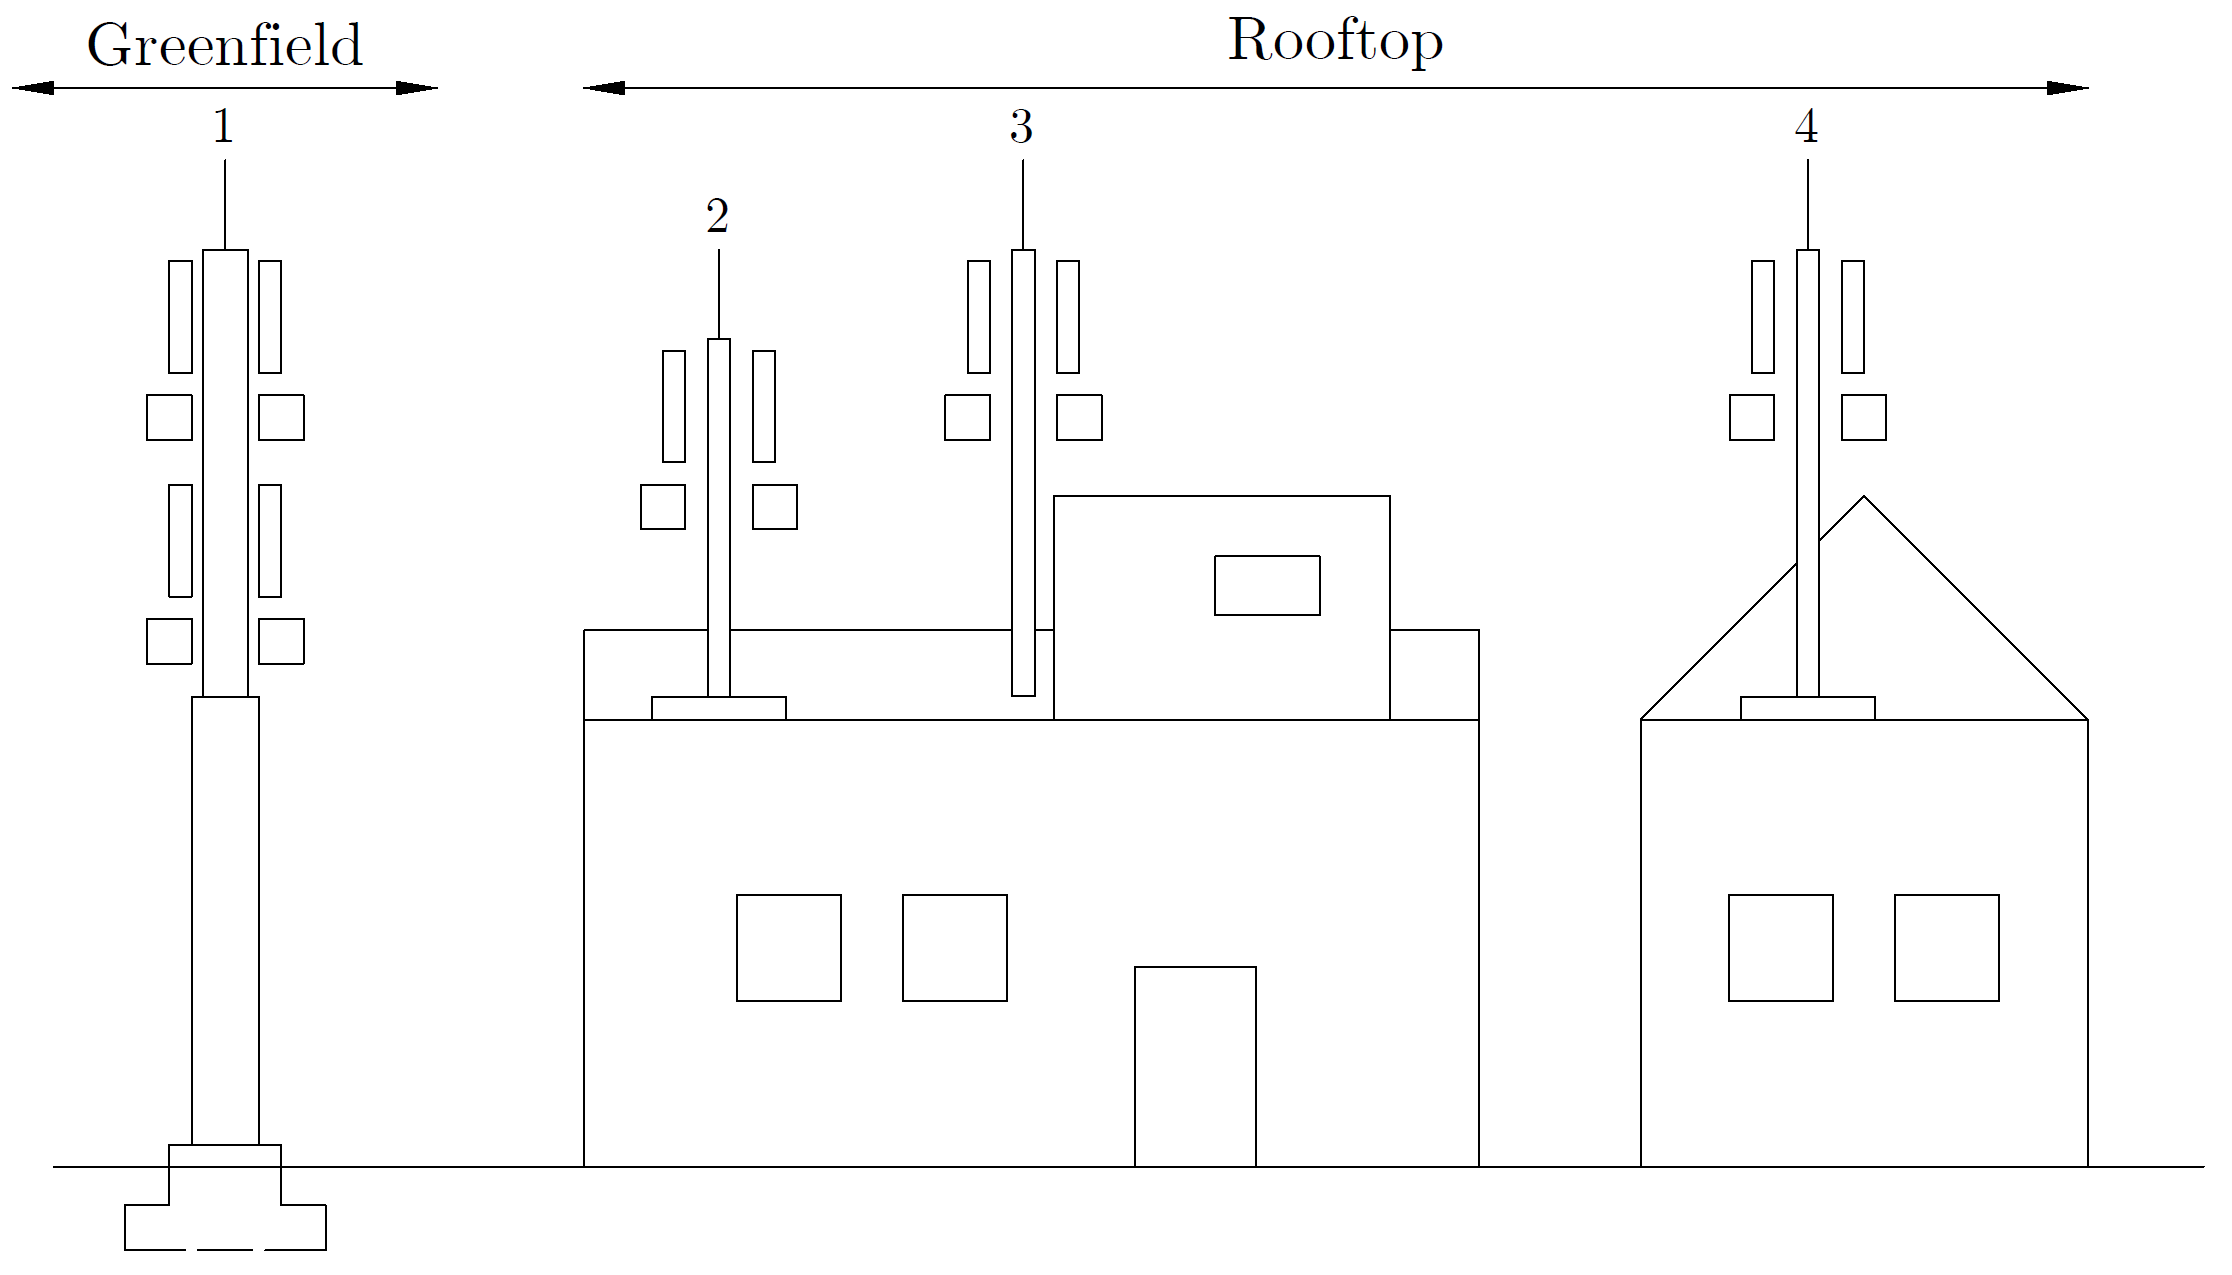
\includegraphics[width=1\textwidth]{dwg/site_classification.PNG}
    \caption{Site Classification (author's own illustration)}
    \label{fig:site_classification}
\end{figure}

\section{Building Information Modeling (BIM)}
\begin{German} 
    BIM wird an verschiedenen Stellen unterschiedlich definiert \cite{astourLehrbuchGrundlagenBIMArbeitsmethode2022}. Nach der Definition der National BIM Services USA steht BIM sowohl für den Modellierungsprozess (Building Information Modelig), das digitale Modell (Building Information Model) als auch für den übergeordnete organisatorische Ablauf (Building Information Management). In Europa verbreiteter ist die Definition nach ISO 19650-1:2018(E), Abschnitt 3.3.14:

    \begin{quote}
        \textbf{Definition:}\\
        use of a shared digital representation of a built asset to faciliate design, constructions and operation processes to form a reliable basis for decisions.
    \end{quote}
        
    Damit ist BIM eine Methodik zur digitalen Planung, Ausführung und Verwaltung von Bauwerken über deren gesamten Lebenszyklus hinweg \cite{astourLehrbuchGrundlagenBIMArbeitsmethode2022}. Zur klaren Unterscheidung wird nachfolgend das Modell als BIM-Modell und das Bearbeitungstool als BIM-Software bezeichnet. Nachfolgend sollen zentrale Erkenntnisse der Literaturanalyse zusammengefasst werden.
\end{German}

\begin{English}
    The term BIM is defined differently \cite{astourLehrbuchGrundlagenBIMArbeitsmethode2022}. According to National BIM Services USA, BIM stands for the modeling process (Building Information Modeling), the digital representation (Building Information Model) and the overarching organisational process (Building Information Management). In Europe, the ISO 19650-1:2018(E) definition in section 3.3.14 is more widespread:

    \begin{quote}
        \textbf{Definition:}\\
        use of a shared digital representation of a built asset to faciliate design, constructions and operation processes to form a reliable basis for decisions.
    \end{quote}

    BIM is therefore a methodology for the digital planning, execution, and management of buildings throughout their entire life cycle \cite{astourLehrbuchGrundlagenBIMArbeitsmethode2022}. For clarity, the digital representation will be referred to as the BIM model, while the processing environment will be referred to as BIM software. The key findings of the literature analysis are summarised below:
\end{English}

\subsection{Characteristics of a BIM Model}
\begin{German}
    Ein BIM-Modell besteht zunächst, wie ein dreidimensionale CAD-Modell auch, aus geometrischen Daten. Zusätzlich zu den geometrischen Daten enthält das BIM-Modell weitere Informationen, die als semantische Eigenschaften bezeichnet werden. Während ein CAD-Modell in der Regel eine Aggregation geometrischer Primitiven (z.B. Punkte, Linien, Flächen) darstellt, setzt sich ein BIM-Modell aus objektbasierten, semantisch angereicherten Bauteilen zusammen. Diese Bauteile verfügen neben ihrer geometrischen Repräsentation über beschreibende Attribute (z.B. Material, Kosten). 
    
    In der Regel sind BIM-Bauteile parametrisch definiert. Ihre Geometrie und Semantik lassen sich über veränderbare Parameter (z.B. Länge, Höhe, Dicke, Typ) steuern. Darüber hinaus können Bauteile sowohl semantisch (inhaltlich) als auch topolgoisch (räumlich) miteinander verknüpfen werden, um funktionale Beziehungen und konstruktive Abhängigkeiten abzubilden.
    
    Aus einem erstellten BIM-Modell lassen sich automatisch 2D-Plandarstellungen (z.B. Grundrisse, Schnitte, Ansichten) sowie Stücklisten und Mengenberechnungen ableiten. Änderungen am Modell werden automatisch in den Plänen abgebildet. Dies ist ein wesentlicher Vorteil gegenüber der konventionellen Planung, bei der Änderungen manuell in den Plänen umgesetzt werden müssen. \cite{astourLehrbuchGrundlagenBIMArbeitsmethode2022} 
\end{German}

\begin{English}
    A BIM model, similar to a three-dimensional CAD model, is initially composed of geometric data. In addition to geometric information, the BIM model incorporates further data referred to as semantic properties. A CAD model is typically constituted of an aggregation of geometric primitives, such as points, lines and surfaces. In contrast, a BIM model is composed of object-based components enriched with semantic information. These components include, in addition to their geometric representation, descriptive attributes such as material or cost.

    BIM components are generally defined parametrically, meaning that both their geometry and semantic properties can be controlled through adjustable parameters such as length, height, thickness, or type. In addition, components can be linked both semantically (i.e., based on functional or categorical relationships) and topologically (i.e., based on spatial or structural connections) in order to represent functional dependencies as well as constructive relationships within the model.

    A completed BIM model allows for the automatic derivation of 2D plan representations (e.g., floor plans, sections, elevations) as well as bills of quantities and material take-offs. Any modifications made to the model are automatically reflected in all associated drawings and documentation. This represents a significant advantage over conventional planning methods, where changes must be implemented manually in each individual plan. \cite{astourLehrbuchGrundlagenBIMArbeitsmethode2022}
\end{English}

\subsection{BIM Terminology}
\begin{German}
    Zur Beschreibung, Bewertung und Vergleichbarkeit von BIM-Anwendungen haben sich eine Reihe standardisierter Begriffe und Kennzahlen etabliert. Sie dienen dazu, den Informationsgehalt und die Entwicklungsstufe von Modellen sowie die Prozesse innerhalb eines BIM-Projekts systematisch zu erfassen. Eine gemeinsame Terminologie schafft dabei die Grundlage für eine eindeutige Kommunikation zwischen allen Projektbeteiligten und unterstützt die konsistente Umsetzung von BIM-Standards. 
    
    Für diese Arbeit sind insbesondere die Begriffe Level of Development (LOD) und Level of Information (LOIN) sowie die Unterscheidung zwischen dem BIM-Anwendungsfall und der BIM-Anwendungsform von Relevanz:
\end{German}

\begin{English}
    A set of standardized terms and key indicators has been established to describe, assess, and compare BIM applications. These serve to systematically capture the information content and level of development of models, as well as the processes within a BIM project. A consistent terminology provides the foundation for clear communication among all project stakeholders and supports the uniform implementation of BIM standards. 
    
    This work places particular emphasis on the concepts of Level of Development (LOD) and Level of Information (LOIN), as well as the distinction between BIM use cases and BIM implementation types:
\end{English}

\setlength{\parindent}{0pt}
\subsubsection{Level of Development (LOD)}

\begin{German}
    Für den Begriff Level of Development (LOD) konnte keine ISO-Definition gefunden werden. Die Non-Profit Organisation BIMForum beschreibt LOD in \textit{2024 Level of Development (LOD) Specification, Part I} wie folgt:

    \begin{quote}
        \textbf{Beschreibung:}\\
        The Level of Development (LOD) Specification is a reference that enables practitioners in the AEC Industry to specify and articulate with a high degree of clarity the content and reliability of Building Information Models (BIMs) at various stages in the design and construction process.\\
        
        \textbf{Note}\\
        LOD is sometimes interpreted as Level of Detail rather than Level of Development. Level of Detail is essentially how much detail is included in the model element. Level of Development is the degree to which the element's geometry has been thought through -- the degree to which project team members may rely on the information when using the model.
    \end{quote}
    
    Level of Development bezeichnet somit den Grad der Ausarbeitung eines Modells in einer spezifischen Projektphase. Der LOD setzt sich zusammen aus dem Level of Geometry (LOG) und dem Level of Infromation (LOI) \cite{astourLehrbuchGrundlagenBIMArbeitsmethode2022}:
\end{German}

\begin{English}
    No official ISO definition could be found for the term Level of Development (LOD). The non-profit organization BIMForum describes LOD in its \textit{2024 Level of Development (LOD) Specification, Part I} as follows:

    \begin{quote}
        \textbf{Description:}\\
        The Level of Development (LOD) Specification is a reference that enables practitioners in the AEC Industry to specify and articulate with a high degree of clarity the content and reliability of Building Information Models (BIMs) at various stages in the design and construction process.\\
        
        \textbf{Note}\\
        LOD is sometimes interpreted as Level of Detail rather than Level of Development. Level of Detail is essentially how much detail is included in the model element. Level of Development is the degree to which the element's geometry has been thought through -- the degree to which project team members may rely on the information when using the model.
    \end{quote}
    
    The Level of Development refers to the extent to which a model element is developed at a specific stage of a project. It consists of two components: the Level of Geometry (LOG), which defines the degree of geometric detail, and the Level of Information (LOI), which specifies the richness of associated non-graphical data \cite{astourLehrbuchGrundlagenBIMArbeitsmethode2022}:
\end{English}

    \begin{equation}
        \text{LOD} = \text{LOG} + \text{LOI}
    \end{equation}
    
 \begin{German}   
    Der LOD wird mit Zahlen zwischen 100 und 500 gekennzeichnet (vgl. Abb. \ref{fig:Level_of_Development}). Dabei nimmt der Detailierungsgrad mit steigender Zahl zu. Mit fortschreitendem Planungsstand nimmt der LOD in der Regel zu.
\end{German}
\begin{English}
    The Level of Development (LOD) is represented by numerical stages ranging from 100 to 500 (cf. Fig. \ref{fig:Level_of_Development}). The level of detail increases with higher LOD stages. As the design progresses, the LOD typically advances accordingly.
\end{English}


    \begin{figure}[h]
        \centering
        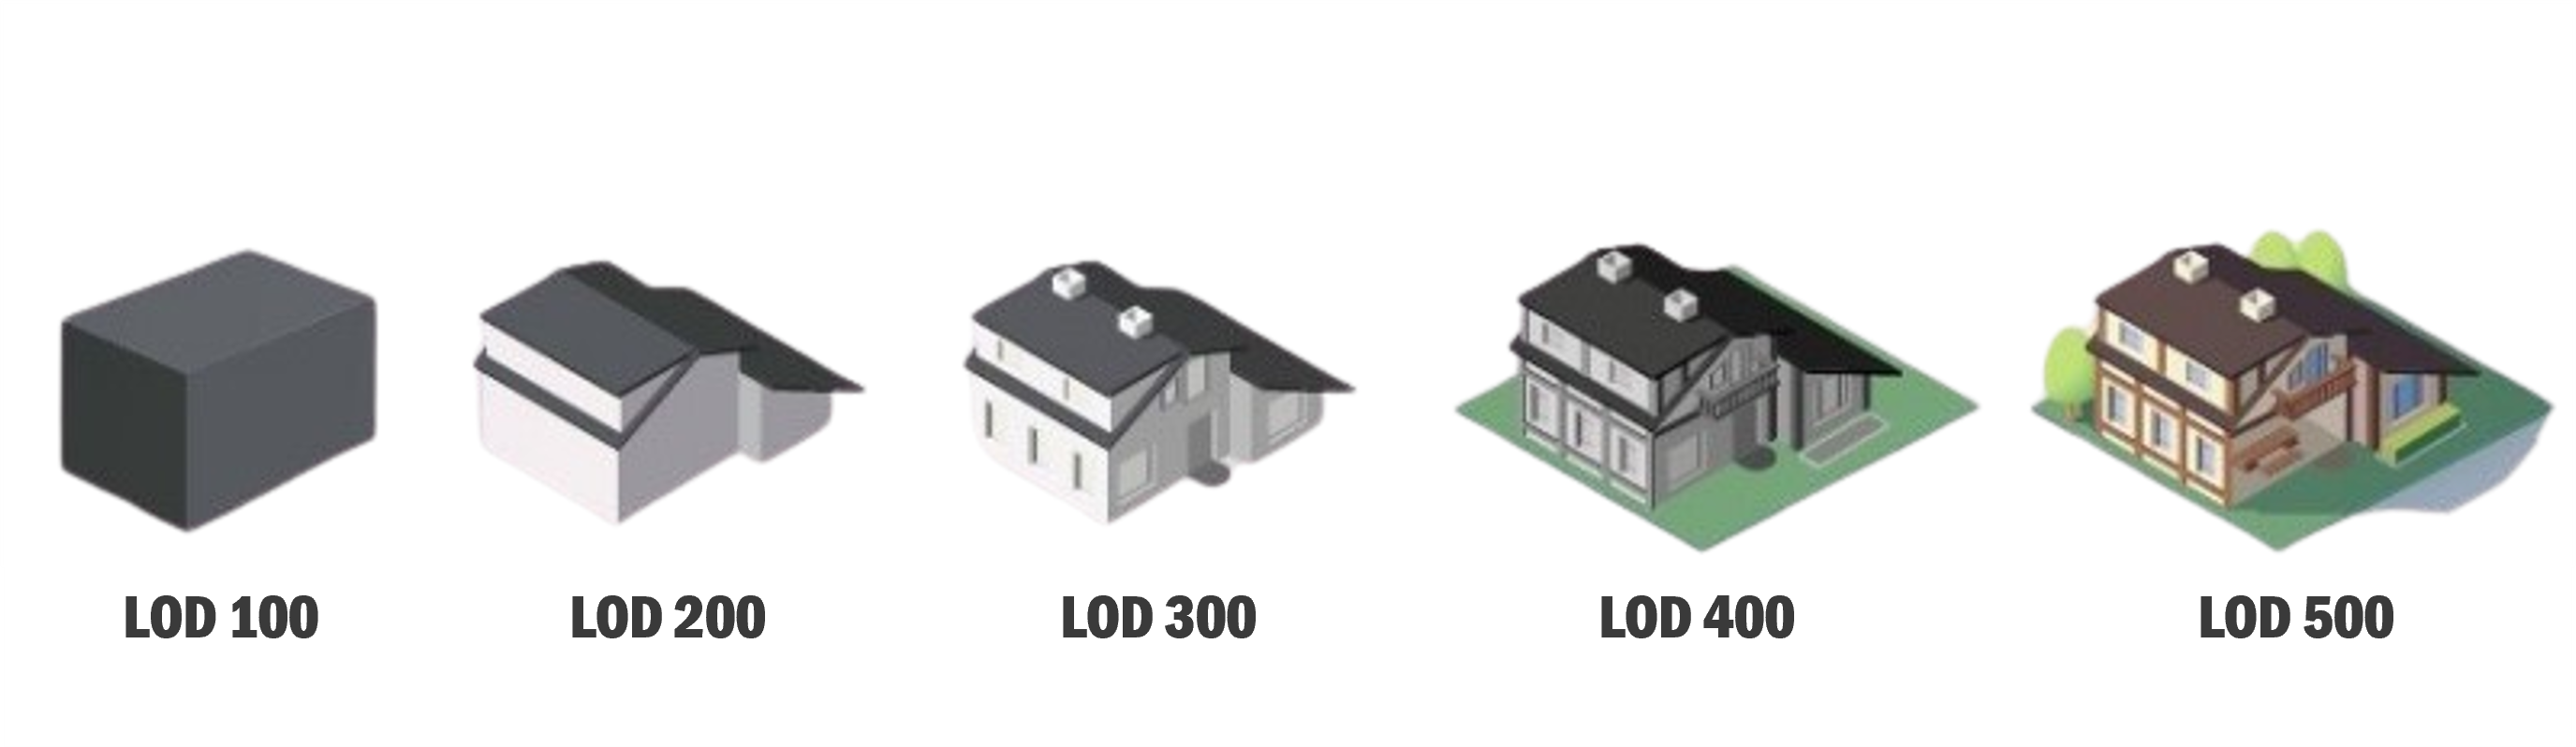
\includegraphics[width=1\textwidth]{images/bim_levels_of_development.png}
        \caption{Level of Development (LOD) \cite{ncircletechBIMLevelDevelopment}}
        \label{fig:Level_of_Development}
    \end{figure}

\subsubsection{Level of Information Need (LOIN)}
\begin{German}
    Der Begriff Level of Information Need (LOIN) wird in der \textit{ISO 19650-1:2018(E), Abschnitt 3.3.16} definiert:
    \begin{quote}
        \textbf{Definition:}\\
        Framework which defines the extent and granularity of information.
    \end{quote}

    Der LOIN beschreibt somit den Umfang und die Granularität der Informationen, die für eine bestimmte Phase benötigt werden. Der LOIN dient als Grundlage für die Festlegung des erforderlichen LOD. Damit soll verhidnert werden, dass ein BIM-Modell unzureichend oder übermässig detailliert beschrieben wird. Letzteres würde den Modellierungsaufwand unnötig erhöhen. Eine übermässige Detaillierung würde den Modellierungsaufwand unnötig erhöhen und die Effizienz im Planungsprozess beeinträchtigen. \cite{astourLehrbuchGrundlagenBIMArbeitsmethode2022}
\end{German}

\begin{English}
    The term Level of Information Need (LOIN) is defined in \textit{ISO 19650-1:2018(E), Section 3.3.16} as:
    \begin{quote}
        \textbf{Definition:}\\
        Framework which defines the extent and granularity of information.
    \end{quote}

    LOIN thus describes the scope and level of detail of information required for a specific project phase. It serves as the basis for determining the appropriate LOD. The objective is to prevent a BIM model from being either insufficiently or excessively detailed. Excessive detailing would unnecessarily increase the modelling effort and impair efficiency in the planning process. \cite{astourLehrbuchGrundlagenBIMArbeitsmethode2022}
\end{English}

\subsubsection{BIM Use Cases}
\begin{German}    
    Der Begriff BIM-Anwendungsfall wird von der Non-Profit-Organisastion buildingSMART International im \textit{BIMcert Handbuch 2024, Abschnitt 3.9.1} wie folgt beschrieben:

    \begin{quote}
        \textbf{Beschreibung:}\\
        BIM-Anwendungsfälle (Use Cases) bezeichnen einen Zweck, für den Daten und Informationen in einem digitalen Bauwerksmodell erstellt und verwendet werden. Ein Use Case beschreibt den Geschäftsfall und das ideale Szenario, einschliesslich der Ziele und Erfolgskriterien für den Informationsaustausch.
    \end{quote}

    Ein BIM-Anwendungsfall beschreibt somit, \textbf{wofür} BIM eingesetzt wird.
\end{German}

\begin{English}
    The term BIM use case is described by the non-profit organization buildingSMART International in its \textit{BIMcert Handbook 2024, Section 3.9.1} as follows:

    \begin{quote}
        \textbf{Description:}\\
        BIM use cases describe the purpose for which data and information are created and used in a digital building model. A use case describes the business case and the ideal scenario, including the objectives and success criteria for information exchange.
    \end{quote}

    A BIM use case thus describes the purpose for which BIM is applied within a specific project or process.
\end{English}

\subsubsection{BIM Implementation Forms}
\begin{German}
    Vier BIM-Anwendungsformen werden von BuildingSMART International in ihrem \textit{BIMcert Handbuch 2024, Abschnitt 2.5.3} beschrieben (vgl. Abb. \ref{fig:BIM_use_cases}). Diese können anhand zweier Dimensionen unterschieden werden \cite{astourLehrbuchGrundlagenBIMArbeitsmethode2022}:

    \begin{enumerate}
        \item \textbf{Reichweite:} Beschreibt den organisatorische Umfang der BIM-Anwendung innerhalb eines Projekts. Die Reichweite entscheidet darüber, ob das Modell lediglich intern genutzt oder über verschiedene Projektbeteiligte hinweg kollaborativ eingesetzt wird.
        \item \textbf{Interoperabilität} Beschreibt die Fähigkeit verschiedener Softwarelösungen und Projektbeteiligter, BIM-Daten unabhängig vom System auszutauschen, zu verstehen und weiterzuverarbeiten.
    \end{enumerate}

    Eine BIM-Anwendungsform beschreibt, \textbf{wie} BIM im Projekt organisatorisch und technisch umgesetzt wird.
    Die Wahl der Anwendungsform ist dabei vom jeweiligen BIM-Anwendungsfall abhängig, da dieser die Anforderungen an Kollaboration und Informationsaustausch bestimmt.
    Grundsätzlich wird der Einsatz von Big Open BIM empfohlen, um eine disziplinübergreifende und softwareunabhängige Zusammenarbeit zu ermöglichen \cite{astourLehrbuchGrundlagenBIMArbeitsmethode2022}.
\end{German}

\begin{English}
    Four BIM implementation forms are described by BuildingSMART International in the BIMcert Manual 2024, Section 2.5.3 (cf. Fig. \ref{fig:BIM_use_cases}). These can be distinguished based on two dimensions \cite{astourLehrbuchGrundlagenBIMArbeitsmethode2022}:
    
    \begin{enumerate}
        \item \textbf{Organisational scope:} Describes the organisational extent of BIM implementation within a project. The scope determines whether the model is used internally only or collaboratively across multiple project participants.
        \item \textbf{Interoperability:} Describes the ability of different software solutions and project stakeholders to exchange, interpret, and further process BIM data independently of the system used.
    \end{enumerate}

    A BIM implementation form describes how BIM is organisationally and technically applied within a project. The choice of an implementation form depends on the specific BIM use case, as it defines the requirements for collaboration and information exchange.
    In general, the use of Big Open BIM is recommended in order to enable interdisciplinary and software-independent cooperation \cite{astourLehrbuchGrundlagenBIMArbeitsmethode2022}.
\end{English}
\setlength{\parindent}{\oldparindent}

\begin{figure}[h]
    \centering
    \resizebox{0.9\linewidth}{!}{%
    \begin{tikzpicture}

        % Define Axis Styles
        \draw[thick,->] (0,0) -- (10,0) node[anchor=west, align=left] {Organisational\\scope};
        \draw[thick,->] (0,0) -- (0,6) node[anchor=south, align=center] {Interoperability};
        \node[anchor=north] at (2.5,0) {little};
        \node[anchor=north] at (7.5,0) {big};
        \node[anchor=south, rotate=90] at (0,1.5) {closed};
        \node[anchor=south, rotate=90] at (0,4.5) {open};

        % Draw Quadrant Lines
        \draw[thick, color={rgb,255:red,150; green,150; blue,150}] (5,0) -- (5,6); % Vertical
        \draw[thick, color={rgb,255:red,150; green,150; blue,150}] (0,3) -- (10,3); % Horizontal

        % Labels for quadrants
        \node at (2.5,4.5) {little open BIM};
        \node at (7.5,4.5) {big open BIM};
        \node at (2.5,1.5) {little closed BIM};
        \node at (7.5,1.5) {big closed BIM};

    \end{tikzpicture}%
    }
    \caption{BIM implementation forms}
    \label{fig:BIM_use_cases}
\end{figure}



\begin{comment}
\subsubsection{BIM Dimensions - optional}
\begin{German}
    Die \textbf{BIM-Dimension} beschreibt die Informationstiefe der Attribute. Sie wird angegeben durch einen Wert zwischen 3D bis 7D. Dabei nimmt der Detailierungsgrad mit steigender Zahl zu. \cite{mayBIMImImmobilienbetrieb2022}
\end{German}
\begin{English}
    The \textbf{BIM dimension} describes the depth of information of the attributes. It is indicated by a value between 3D and 7D. The level of detail increases with increasing number. \cite{mayBIMImImmobilienbetrieb2022}
\end{English}

% table
\begin{table}[h]
    \centering
    \renewcommand{\arraystretch}{1.2} % Adjust row height for better readability
    \setlength{\tabcolsep}{5pt} % Adjust column spacing
    \resizebox{\textwidth}{!}{ % Resizes table to fit within text width
    \begin{tabular}{|c|l|l|}
        \hline
        \textbf{Dimension} & \textbf{Additional Attributes} & \textbf{Use Cases} \\
        \hline
        \textbf{3D} & None & Geometric modeling \\
        \hline
        \textbf{4D} & Time & Construction scheduling, project phases \\
        \hline
        \textbf{5D} & Cost & Quantity takeoff, pricing, budgeting \\
        \hline
        \textbf{6D} & Efficiency \& Sustainability & Energy performance, lifecycle assessment \\
        \hline
        \textbf{7D} & Facility management & Operations, maintenance, asset tracking \\
        \hline
    \end{tabular}
    }
    \caption{BIM Dimensions and Information Depth}
    \label{tab:BIM_dimensions}
\end{table}

\subsubsection{BIM Maturity Level - optional}
\begin{German}
    Der \textbf{BIM-Reifegrad} ist ein Qualitätsmass, das beschreibt, wie systematisch und umfassend BIM in einem Unternehmen oder Projekt implementiert ist. Der Schwerpunkt liegt auf der Vernetzung von Daten, der Standardisierung sowie der Zusammenarbeit zwischen den Beteiligten. Gemäß VDI 2552 werden die folgenden vier Reifegrade unterschieden: \cite{astourLehrbuchGrundlagenBIMArbeitsmethode2022,eichlerBIMcertHandbuchGrundlagenwissen2023}\\
\end{German}
\begin{English}
    The \textbf{BIM maturity level} is a quality measure that describes how systematically and comprehensively BIM is implemented in a company or project. The focus is on data networking, standardization, and collaboration between the participants. According to VDI 2552, the following four maturity levels are distinguished: \cite{astourLehrbuchGrundlagenBIMArbeitsmethode2022,eichlerBIMcertHandbuchGrundlagenwissen2023}\\
\end{English}

\begin{table}[h]
    \centering
    \renewcommand{\arraystretch}{1.2} % Adjust row height for better readability
    \setlength{\tabcolsep}{5pt} % Adjust column spacing
    \begin{tabularx}{\textwidth}{|c|l|X|}
        \hline
        \textbf{Level} & \textbf{BIM Usage} & \textbf{Description}  \\
        \hline
        \textbf{0} & None &  Traditional 2D CAD drafting is used with no object-based modeling or intelligent data sharing. Collaboration is minimal, and document exchange is paper-based or in simple file formats. \\
        \hline
        \textbf{1} & None &  Combination of 2D and 3D CAD tools. While 3D models may be used internally, there is no standardized collaboration between different disciplines. Data exchange remains file-based without integrated workflows. \\
        \hline
        \textbf{2} & Collaborative &  Different disciplines work on their own BIM models, which are then shared and combined at specific project stages. Collaboration is structured, but data exchange is still semi-automated, requiring manual coordination. Lifecycle phases are considered separately. \\
        \hline
        \textbf{3} & Integrated & All disciplines collaborate in a fully connected and shared BIM environment. A single, integrated model covers the entire building lifecycle, from design to operation. Automated data exchange and real-time collaboration enable seamless workflows. \\
        \hline
    \end{tabularx}
    \caption{BIM Stages and Their Characteristics}
    \label{tab:BIM_stages}
\end{table}

\subsection{BIM Management - optional}
\begin{German}
    Das \textbf{BIM-Management} beinhaltet die strategische und operative Steuerung von BIM. Es sollen damit Workflows standardisiert und die Zusammenarbeit verbessert werden. In diesem Unterkapitel sollen drei Werkzeuge vorgestellt werden (vgl. \ref{fig:BIM_management}), auf die in der Fallstudie zurückgegriffen wird.
\end{German}
\begin{English}
    \textbf{BIM management} involves the strategic and operational control of BIM. The aim is to standardize workflows and improve collaboration. In this subchapter, three tools will be presented (see \ref{fig:BIM_management}), which will be used in the case study.
\end{English}

\subsubsection{Exchange Information Requirements (EIR)}
\begin{German}
    Die \textbf{Auftraggeber-Informations-Anforderungen (AIA)} entsprechen einem auf BIM zugeschnittenen Lastenheft. Sie beschreiben, warum welche Information wann benötigt werden. Sie definieren die Anforderungen des Auftraggebers an BIM-Prozesse, Daten und Zusammenarbeit über den gesamten Projektlebenszyklus. Dazu gehören Vorgaben zu Modellstruktur, Detaillierungsgrad, Datenaustauschformaten, Verantwortlichkeiten und Kollaborationsmethoden. \cite{astourLehrbuchGrundlagenBIMArbeitsmethode2022}
\end{German}
\begin{English}
    The \textbf{Exchange Information Requirements (EIR)} correspond to a specification tailored to BIM. They describe why which information is needed when. They define the client's requirements for BIM processes, data, and collaboration throughout the entire project life cycle. This includes specifications for model structure, level of detail, data exchange formats, responsibilities, and collaboration methods. \cite{astourLehrbuchGrundlagenBIMArbeitsmethode2022}
\end{English}

\subsubsection{BIM Execution Plan (BEP)}
\begin{German}
    Der \textbf{BIM-Abwicklungsplan (BAP)} entspricht einem auf BIM zugeschnittenen Pflichtenheft. Er beschreibt, wie die Anforderungen aus dem \textbf{Auftraggeber-Informations-Anforderungen (AIA)} vom Auftragnehmer im Projekt umgesetzt werden. \cite{astourLehrbuchGrundlagenBIMArbeitsmethode2022}
\end{German}
\begin{English}
    The \textbf{BIM Execution Plan (BEP)} corresponds to a specification tailored to BIM. It describes how the requirements from the \textbf{Employer's Information Requirements (EIR)} are implemented by the contractor in the project. \cite{astourLehrbuchGrundlagenBIMArbeitsmethode2022}
\end{English}

\subsubsection{BIM Modeling Guidelines}
\begin{German}
    Die \textbf{BIM-Modellierungsrichtlinien} legen fest, wie ein BIM-Modell aufgebaut und strukturiert sein soll. Dafür werden Standards, Methoden und Anforderungen für die Erstellung und Verwaltung definiert. Sie sorgen für einheitliche Datenstrukturen, bessere Zusammenarbeit und eine hohe Modellqualität. Typischerweise werden die Modelleriungsrichtlinien im BAP definiert oder referenziert. \cite{astourLehrbuchGrundlagenBIMArbeitsmethode2022}
\end{German}
\begin{English}
    The \textbf{BIM modeling guidelines} define how a BIM model should be structured and organized. For this purpose, standards, methods, and requirements for creation and management are defined. They ensure uniform data structures, better collaboration, and high model quality. Typically, the modeling guidelines are defined or referenced in the BEP. \cite{astourLehrbuchGrundlagenBIMArbeitsmethode2022}
\end{English}

\begin{figure}[h]
    \centering
    \begin{tikzpicture}[
        node distance=3.2cm, % Distance between nodes
        every node/.style={draw, minimum width=2.5cm, minimum height=1.5cm, align=center}, % Box styling
        every path/.style={thick, -stealth} % Arrow styling
        ]
        
        % Define nodes
        \node (EIR) {EIR};
        \node (BEP) [right of=EIR] {BEP};
        \node (Modelling) [right of=BEP] {BIM \\ Modelling \\ Guidelines};
        \node (BIM) [right of=Modelling] {BIM Modell};

        % Draw arrows
        \draw (EIR) -- (BEP);
        \draw (BEP) -- (Modelling);
        \draw (Modelling) -- (BIM);
        
        % Draw additional curved arrow from EIR to BIM Modell
        \draw[->] (BEP.north) |- ([yshift=0.5cm] BIM.north) -| (BIM.north);

    \end{tikzpicture}
    \caption{Simplified BIM Management Process Flow}
    \label {fig:BIM_management}
\end{figure}
\end{comment}


\section{Scan-to-BIM}
\begin{German}
    Umbauprojekte werden in der Schweizer Bauwirtschaft immer wichtiger. Die jährlichen Bauausgaben für Neubauprojekte sind gegenüber 1980 beinahe gleich geblieben \cite{bundesamtfuerstatstikBauausgabenNachArt}. Die Investitionen in Erneuerungen hat sich in der gleichen Periode über verdreifacht. 
    
    Zusätzlich ist bei privaten Bestandsbauten die Dokumentation häufig lückenhaft \cite{dewolfCircularBuiltEnvironment,kadenLeitfadenGeodaesieUnd}. Besonders ältere Gebäude verfügen oft nur über unvollständige oder veraltete Planunterlagen. Zwar lassen sich in Gemeindearchiven häufig Baueingabepläne auffinden, diese dokumentieren jedoch den ursprünglichen Bauzustand, sind oft überholt und in niedrigem Detailierungsgrad.

    In der Schweiz wurden 81,5\,\% der Gebäude vor dem Jahr 2000 errichtet \cite{bundesamtfuerstatstikBauperiode}. Falls Planunterlagen vorhanden sind, liegen diese in der Regel ausschliesslich in Papierform vor. Selbst bei neueren Gebäuden sind digitale CAD- oder BIM-Dateien häufig nicht verfügbar. Da Planer aus Haftungsgründen ungern editierbare Daten herausgeben, erhalten Eigentümer meist nur Papierpläne, was ohne explizite vertragliche Regelung rechtlich zulässig ist \cite{bundschwBauenRechtenUnd}. In solchen Fällen bietet Scan-to-BIM eine Möglichkeit zur nachträglichen Digitalisierung von Bauwerken. Nachfolgend soll der Arbeitsablauf von Scan-to-BIM untersucht werden.

    Es konnten dafür keine wissenschaftliche Fachbücher identifiziert werden, die Scan-to-BIM als Hauptthema behandelten. Es wurden daher die wissenschaftlichen Publikationen \cite{wangApplicationOrientedScantoBIM2019, badenkoSCANTOBIMMETHODOLOGYADAPTED2019, borrusoProceduralPointCloud2023, rashdiScanningTechnologiesBuilding2022} herangezogen. Die darin beschriebenen Arbeitsabläufe bestanden aus drei bis sechs Arbeitsschritten (vgl. Abb. \ref{tab:scan-to-bim_workflows}).
    
    Aus der analysierten Literatur wurde ein eigener, konsolidierter Arbeitsablauf abgeleitet. Dieser umfasst die Arbeitsschritte Data Acquisition (1), Preprocessing (2), Geometric Reconstruction (3), Semantic Segmentatin (4) sowie Modeling (5) (siehe Abb. \ref{fig:Scan_to_BIM_workflow}). Die einzelnen Arbeitsschritte werden nachfolgend zusammengefasst und systematisch erläutert.
\end{German}

\begin{English}
    Refurbishments are becoming increasingly important in the Swiss construction industry. Since 1980, annual construction expenditures for new building projects have remained nearly constant \cite{bundesamtfuerstatstikBauausgabenNachArt}, while investments in building renewals have more than tripled over the same period. 
    
    In addition, documentation of privately owned existing buildings is frequently incomplete \cite{dewolfCircularBuiltEnvironment, kadenLeitfadenGeodaesieUnd}. This applies especially to older structures, which often possess only outdated or partial sets of construction drawings. While permit drawings can often be located in municipal archives, these typically reflect the original design state, are often outdated, and exhibit a low level of detail.
    
    In Switzerland, 81.5\,\% of buildings were constructed before the year 2000 \cite{bundesamtfuerstatstikBauperiode}. Where construction documents are available, they are typically only accessible in paper form. Even for more recent buildings, digital CAD or BIM files are often unavailable. Due to liability concerns, planners are generally reluctant to provide editable data. As a result, building owners are usually given printed plans only, a practice that is legally permissible in the absence of an explicit contractual agreement \cite{bundschwBauenRechtenUnd}. In such cases, Scan-to-BIM offers a viable solution for the retrospective digitization of buildings. The following section examines the workflow of the Scan-to-BIM process.

    No academic textbooks could be identified that treat Scan-to-BIM as a primary subject. Therefore, the analysis draws on selected academic publications \cite{wangApplicationOrientedScantoBIM2019, badenkoSCANTOBIMMETHODOLOGYADAPTED2019, borrusoProceduralPointCloud2023, rashdiScanningTechnologiesBuilding2022}, in which the described workflows consist of three to six steps (cf. Tab. \ref{tab:scan-to-bim_workflows}).

    Based on the reviewed literature, a consolidated workflow has been derived. It comprises the following five steps: Data Acquisition (1), Preprocessing (2), Geometric Reconstruction (3), Semantic Segmentation (4), and Modeling (5) (see Fig. \ref{fig:Scan_to_BIM_workflow}). The individual steps are summarized and systematically discussed in the following section.
\end{English}

\begin{table}[h]
    \centering
    \begin{tabular}{p{2cm} p{9cm}}
        \textbf{Publication} & \textbf{Proposed steps} \\
        \hline
        \cite{wangApplicationOrientedScantoBIM2019} & 1. Identification of information requirements \\
                & 2. Determination of required scan data quality \\
                & 3. Scan data acquisition \\
                & 4. As-is BIM reconstruction \\
        \hline
        \cite{badenkoSCANTOBIMMETHODOLOGYADAPTED2019} & 1. Classification of considered elements \\
                & 2. Determination of required level of detail \\
                & 3. Scan data acquisition \\
                & 4. Point cloud registration and segmentation \\
                & 5. As-built BIM model generation \\
                & 6. Analysis \\
        \hline
        \cite{borrusoProceduralPointCloud2023} & 1. Data acquisition \\
                & 2. Data preprocessing \\
                & 3. Modeling \\
        \hline
        \cite{rashdiScanningTechnologiesBuilding2022} & 1. Data capture \\
                & 2. Semantic segmentation \\
                & 3. BIM model \\
    \end{tabular}
    \caption{Proposed Scan-to-BIM Worksflows in Literature}
    \label{tab:scan-to-bim_workflows}
\end{table}


\begin{figure}[h]
    \centering
    \begin{tikzpicture}[
        process/.style={draw, rectangle, minimum width=2.8cm, minimum height=1.2cm, align=center},
        every path/.style={thick, -stealth}
    ]
        % Prozessboxen nebeneinander
        \node (step1) [process] at (0,0) {Data Acquisition\\(1)};
        \node (step2) [process, right=0.5cm of step1] {Preprocessing\\(2)};
        \node (step3) [process, right=0.5 of step2] {Geometric\\Reconstruction\\(3)};
        \node (step4) [process, below=0.3 of step3] {Semantic\\Segmentation\\(4)};
        \node (step5) [process, left=0.5 of step4] {Modeling\\(5)};
        
        % Pfeile zwischen den Schritten
        \draw[->] (step1) -- (step2);
        \draw[->] (step2) -- (step3);
        \draw[->] (step3) -- (step4);
        \draw[->] (step4) -- (step5);

    \end{tikzpicture}
    \caption{Proposed Scan-to-BIM workflow based on literature synthesis}
    \label{fig:Scan_to_BIM_workflow}
\end{figure}

\setlength{\parindent}{0pt}
\subsection{Data Acquisition}
\begin{German}
    Die Datenakquise erfolgt mittels Reality-Capture. Dabei wird ein physisches Objekt mithilfe von Sensoren digital erfasst und repräsentiert. Für Scan-to-BIM werden zwei Haupttechnologien verwendet:
    
    \begin{itemize}
        \item \textbf{Light Detection and Ranging (LiDAR):} LiDAR ist ein aktives, direktes Messverfahren zur Distanzbestimmung. Ein Emitter sendet Laserimpulse aus, die von Objekten reflektiert und von einem Detektor empfangen werden. Aus der gemessenen Laufzeit wird die Entfernung berechnet. Als natives Ausgabeformat wird direkt eine Punktwolke erzeugt. \cite{rashdiScanningTechnologiesBuilding2022}
        \item \textbf{Photogrammetrie:} Photogrammetrie ist ein passives, indirektes Messverfahren, das auf der Auswertung überlappender Fotos aus verschiedenen Blickwinkeln basiert. Aus Bildgeometrie und Perspektivunterschieden können Punktwolken oder Meshes rekonstruiert werden. \cite{rashdiScanningTechnologiesBuilding2022}
    \end{itemize}

    LiDAR hat gegenüber Photogrammetrie eine meist höhere Genauigkeit und eignet sich ideal für die Erfassung von Innenräumen sowie bei schlechten Lichtverhältnissen. Photogrammetrie hingegen erfordert keine kostspielige Spezialhardware und stellt damit eine vergleichsweise kostengünstige Alternative dar. Sie wird häufig in Kombination mit Drohnen zur Erfassung von Aussenfassaden eingesetzt. \cite{rashdiScanningTechnologiesBuilding2022}
    
    Die folgenden Formate werden häufig als digitale Repräsentationen verwendet:

    \begin{itemize}
        \item \textbf{Punktwolke:} Eine Punktwolke ist eine Menge von Punkten im dreidimensionalen Raum. Jeder Punkt repräsentiert eine Oberflächenposition \((x, y, z)\) des gescannten Objekts. Neben der Position können den Punkten weitere Attribute wie Farbwerte (r, g, b) oder ein Normalenvektor \((n_x, n_y, n_z)\) zugeordnet sein. Der Normalenvektor beschreibt die Ausrichtung der Oberfläche an der jeweiligen Punktposition und dient vielen Algorithmen als Inputparameter. Im Gegensatz zu Voxel-Grids, dem dreidimensionale Pendant zu einem 2D-Bild, haben die Punkte keine Gitterstruktur. Sie sind strukturfrei, was sie rechnerisch aufwendiger in der Verarbeitung macht. Punktwolken eignen sich besonders gut für präzise Analysen. \cite{liu3DPointCloud2021}
        \item \textbf{Mesh:} Ein Mesh ist eine flächenhafte 3D-Repräsentation eines Objekts, die aus einer Menge von Eckpunkten (Vertices) sowie deren Verbindungen (Kanten und Flächen) besteht. Meist werden die Flächen als Dreiecke definiert, wodurch ein sogenanntes Dreiecksnetz entsteht. Meshes eignen sich besonders gut für realistische Visualisierungen. \cite{borrusoProceduralPointCloud2023}
    \end{itemize}

    Im weiteren Verlauf liegt der Schwerpunkt auf der Analyse von Punktwolken. Zentrale Qualitätsmetriken sind:

    % Genauigkeit = Accuracy
    % Präzision = Precision
    % Richtigkeit = Trueness
    % Punktdichte = Point Density
    % Auflösung = Resolution
    % Abdeckung = Coverage

    \begin{itemize}
        \item \textbf{Präzision:} Bezeichnet die Wiederholgenauigkeit von Messungen und damit die Konsistenz einzelner Messwerte. \cite{wieserKursGeodaetischeMesstechnik}
        
        \item \textbf{Richtigkeit:} Gibt an, wie stark der Mittelwert mehrerer Messungen vom wahren Wert abweicht. \cite{wieserKursGeodaetischeMesstechnik}
        
        \item \textbf{Genauigkeit:} Beschreibt die Abweichung einer einzelnen Messung vom wahren Wert und ergibt sich aus dem Zusammenspiel von Präzision und Richtigkeit. \cite{wieserKursGeodaetischeMesstechnik}
        
        \item \textbf{Abdeckung:} Gibt an, wie vollständig der zu erfassende Bereich durch die Punktwolke repräsentiert wird. Sie ist ein Mass für die räumliche Vollständigkeit. \cite{wieserKursGeodaetischeMesstechnik}
        
        \item \textbf{Punktdichte:} Gibt die Anzahl der erfassten Messpunkte pro Flächeneinheit an und ist ein Mass für die Detailtiefe der Punktwolke. \cite{wieserKursGeodaetischeMesstechnik}
        
        \item \textbf{Auflösung:} Bezeichnet den kleinsten räumlichen Abstand, den das Sensorsystem noch unterscheiden kann. Sie bestimmt, wie fein Details in der Punktwolke abgebildet werden können. \cite{wieserKursGeodaetischeMesstechnik}
    \end{itemize}

\end{German}

\begin{English}
    Data acquisition is done using reality capture. A physical object is digitally captured and represented using sensors. Two main technologies are used for Scan-to-BIM:

    \begin{itemize}
        \item \textbf{Light Detection and Ranging (LiDAR):} LiDAR is an active, direct measurement method for determining distance. The emitter emits laser pulses, which are reflected by objects and received by a detector. The distance is calculated from the measured time of flight. The generation of a point cloud is effected directly as the native output format. \cite{rashdiScanningTechnologiesBuilding2022}
        \item \textbf{Photogrammetry:} Photogrammetry is a passive, indirect measurement method based on the evaluation of overlapping photographs from different perspectives. It is possible to reconstruct point clouds or meshes from image geometry and perspective differences. \cite{rashdiScanningTechnologiesBuilding2022}
    \end{itemize}

    LiDAR is generally considered to be more precise than photogrammetry, and it is particularly well-suited for capturing indoor environments and in conditions where lighting is suboptimal. Conversely, photogrammetry does not necessitate the procurement of costly, specialised hardware, thus rendering it a comparatively cost-effective alternative. Its utilisation in conjunction with drones to capture exterior facades is a common practice. \cite{rashdiScanningTechnologiesBuilding2022}

    The following formats are frequently utilised as digital representations:

    \begin{itemize}
        \item \textbf{Point Cloud:} A point cloud is defined as a set of points in three-dimensional space. Each point corresponds to a surface position \((x, y, z)\) of the scanned object. In addition to the position, further attributes such as colour values (r, g, b) or a normal vector \((n_x, n_y, n_z)\) can be assigned to the points. The normal vector delineates the orientation of the surface at the respective point position and functions as an input parameter for numerous algorithms. In contradistinction to voxel grids, which can be considered the three-dimensional counterpart to a 2D image, the points have no grid structure. The absence of structure renders them more complex to process computationally. Point clouds have been demonstrated to be a particularly suitable data structure for precise analyses. \cite{liu3DPointCloud2021}
        \item \textbf{Mesh:} A mesh is defined as a planar three-dimensional representation of an object that consists of a set of corner points (vertices) and their connections (edges and faces). The surfaces are typically delineated as triangles, thus resulting in what is referred to as a triangular mesh. Meshes are particularly well-suited to realistic visualisations. \cite{borrusoProceduralPointCloud2023}
    \end{itemize}

    The subsequent analysis focuses on point clouds. The central quality metrics are as follows:

    \begin{itemize}
        \item \textbf{Precision:} Describes the repeatability of measurements and thus the consistency of individual values. \cite{wieserKursGeodaetischeMesstechnik}
        
        \item \textbf{Trueness:} Indicates how much the mean of multiple measurements deviates from the actual (true) value. \cite{wieserKursGeodaetischeMesstechnik}
        
        \item \textbf{Accuracy:} Refers to the deviation of a single measurement from the true value and results from the combination of precision and trueness. \cite{wieserKursGeodaetischeMesstechnik}
        
        \item \textbf{Coverage:} Describes how completely the area or object of interest is represented by the point cloud. It serves as a measure of spatial completeness. \cite{wieserKursGeodaetischeMesstechnik}
        
        \item \textbf{Point density:} Indicates the number of points captured per unit area and reflects the level of detail represented in the point cloud. \cite{wieserKursGeodaetischeMesstechnik}
        
        \item \textbf{Resolution:} Defines the smallest spatial distance that a sensor system can distinguish. It determines how finely details can be resolved within the point cloud. \cite{wieserKursGeodaetischeMesstechnik}
    \end{itemize}

\end{English}
\setlength{\parindent}{\oldparindent}

% Kongruenztransformation = Rigid Transformation
% Grobregistrierung = Coarse Registration
% Feinregistrierung = Fine Registration

\subsection{Preprocessing}
\begin{German}
    Im Preprocessing wird die Punktwolke für weiterführende Analysen vorbereitet. Oft werden folgende Schritte durchgeführt:
\end{German}

\begin{English}
    In preprocessing, the point cloud is prepared for further analyses. The following steps are often carried out:
\end{English}

\subsubsection{Registration}
\begin{German}
    Registrierung ist der Prozess, bei dem mehrere Punktwolken aus ihren jeweiligen Scanner-Koordinatensystemen (SCS) durch Transformationen in ein gemeinsames lokales Koordinatensystem (LCS) überführt und zueinander ausgerichtet werden. Ziel ist es, eine zusammenhängende, vollständige Punktwolke zu erzeugen, in der alle Teilbereiche korrekt zueinander positioniert sind. \cite{voordendagKursGeodaetischeMesstechnik}
\end{German}

\begin{English}
    Registration is the process of transforming multiple point clouds from their own scanner coordinate systems (SCS) into a unified local coordinate system (LCS), followed by the alignment of these point clouds with each other. The objective is to generate a coherent, complete point cloud in which all sub-areas are correctly positioned in relation to each other. \cite{voordendagKursGeodaetischeMesstechnik}
\end{English}

\subsubsection{Georeferencing}
\begin{German}
    Die Georeferenzierung ist der Prozess, bei dem eine Punktwolke aus einem lokalen Koordinatensystem (LCS) in ein übergeordnetes, globales Koordinatensystem (GCS) überführt wird. Ziel ist es, die Punktwolke räumlich korrekt in Bezug auf reale Weltkoordinaten zu verorten, sodass sie mit anderen Geodaten kombiniert und weiterverwendet werden kann. Für die Georeferenzierung werden häufig Referenzpunkte, s.g. Ground Control Points (GCPs), verwendet. Diese sind markante Punkte in der realen Welt, deren Koordinaten bekannt sind. Die Punktwolke wird dann über eine Helmert-Transformation (Translation, Rotation, Skalierung) in das GCS überführt. Die Genauigkeit der Georeferenzierung hängt von der Anzahl und Geometrie der GCPs ab. \cite{voordendagKursGeodaetischeMesstechnik}
\end{German}

\begin{English}
    Georeferencing is the process of converting a point cloud from a local coordinate system (LCS) into a global coordinate system (GCS). The objective is to accurately position the point cloud in relation to real-world coordinates, facilitating its integration with other geodata and enabling further utilisation. Reference points, designated as ground control points (GCPs), are frequently employed for the purpose of georeferencing. These are salient points in the real world whose coordinates are known. The point cloud is then transferred to the GCS using a Helmert transformation (translation, rotation, scaling). The precision of georeferencing is contingent upon the quantity and configuration of the GCPs. \cite{voordendagKursGeodaetischeMesstechnik}
\end{English}

\subsubsection{Filtering}
\begin{German}
    Punktwolken entahlten häufig unerwünschte Punkte, die die Qualität der Daten beeinträchtigen. Diese können beispielsweise durch Messrauschen, Ausreisser oder unerwünschte Objekte entstehen. Die Filterung dient dazu, die Punktwolke von solch unerwünschten Punkten zu bereiningen. Folgende Filter werden häufig eingesetzt:

    \begin{enumerate}
        \item \textbf{Rauschfilter:} Rauschen bezeichnet zufällige, kleinräumige Abweichungen der Messpunkte von ihrer tatsächlichen Position. Es kann durch Sensorrauschen, ungünstige Oberflächeneigenschaften oder äussere Einflüsse wie Lichtverhältnisse entstehen. Um die Qualität der Punktwolke zu verbessern, werden Rauschfilter eingesetzt, die diese Abweichungen reduzieren oder betroffene Punkte entfernen. \cite{liu3DPointCloud2021}\\
        \textit{Beispiel: Moving Least Squares Filter (MLS)}
        
        \item \textbf{Ausreisserfilter:} Ausreisser sind einzelne Messpunkte, deren Lage signifikant von der sie umgebenden Punktverteilung abweicht und die nicht zur tatsächlichen Objektgeometrie gehören. Sie entstehen häufig durch Messfehler, Reflexionen oder Störungen während der Datenerfassung. Zur Verbesserung der Datenqualität werden Ausreisserfilter eingesetzt, die solche Punkte erkennen und entfernen. \cite{liu3DPointCloud2021}\\
        \textit{Beispiel: Statistical Outlier Removal Filter (SOR)}
    \end{enumerate}
\end{German}

\begin{English}
    Point clouds frequently contain undesirable points that can compromise the integrity of the data. Such aberrations may be attributed to measurement noise, outliers, or the presence of unwanted objects. Filtering is employed to eliminate such undesirable points from the point cloud. The following filters are frequently utilised:

    \begin{enumerate}
        \item \textbf{Noise Filter:} Noise is defined as random, small-scale deviations of the measuring points from their actual position. The phenomenon may be attributed to sensor noise, unfavourable surface properties or external influences such as lighting conditions. In order to enhance the quality of the point cloud, the implementation of noise filters is a common practice, with the objective of reducing these deviations or removing the points affected. \cite{liu3DPointCloud2021}\\
        \textit{Example: Moving Least Squares Filter (MLS)}
        
        \item \textbf{Outlier Filter:} Outliers are defined as individual measuring points whose position deviates significantly from the surrounding point distribution and which do not belong to the actual object geometry. Errors in measurement, reflections, or interference during data acquisition are frequently the underlying cause. In order to enhance the quality of the data, the implementation of outlier filters is a common practice, with the objective of identifying and eliminating such points. \cite{liu3DPointCloud2021}\\
        \textit{Example: Statistical Outlier Removal Filter (SOR)}
    \end{enumerate}
\end{English}

\subsubsection{Downsampling}
\begin{German}
    Downsampling bezeichnet Verfahren zur gezielten Reduktion der Punktanzahl innerhalb einer Punktwolke. Die geometrisch wesentlichen Strukturen soll dabei erhalten bleiben. Ziel ist es, die Datenmenge zu verringern, um die Effizienz der anschliessenden Punktwolkenverarbeitung zu steigern. \cite{liu3DPointCloud2021}\\
    \textit{Beispiel: Voxel Grid Downsampling, Farthest Point Sampling (FPS), Normal Space Sampling (NSS)}
\end{German}

\begin{English}
    Downsampling is a process for the targeted reduction of the number of points within a point cloud. The geometrically essential structures should be retained. The objective is to minimise the data volume to enhance the subsequent point cloud processing efficiency. \cite{liu3DPointCloud2021}\\
    \textit{Example: Voxel Grid Downsampling, Farthest Point Sampling (FPS), Normal Space Sampling (NSS)}
\end{English}
  

\subsection{Geometric Reconstruction}
\begin{German}
    Die geometrische Rekonstruktion beschreibt den Prozess, bei dem aus der Punktwolke ein 3D-Modell erstellt wird. Dabei werden die relevanten geometrischen Strukturen des gescannten Objekts identifiziert und in eine geeignete 3D-Repräsentation überführt. Die geometrische Rekonstruktion kann in zwei Hauptkategorien unterteilt werden:

    \begin{enumerate}
        \item \textbf{Regelbasierte Methoden:} Diese Methoden extrahieren geometrische Primitive anhand vorgegebener Merkmale aus einer Punktwolke. Sie folgen klar definierten Algorithmen. Diese Methoden funktionieren gut bei sauberen, strukturierten Punktwolken. \cite{fangScantoBIMtoSimAutomatedReconstruction2025}\\
        \textit{Beispiel: RANSAC, PolyFit}

        \item \textbf{Lernbasierte Methoden:} Diese Methoden extrahieren geometrische Primitive anhand selbst gelernter Merkmale aus einer Punktwolke. Dafür werden grosse annotierte Trainingsdatensätze benötigt. Sie sind flexibler und können auch bei unstrukturierten Punktwolken eingesetzt werden. Diese Methoden sind jedoch rechenintensiver und benötigen mehr Zeit für die Verarbeitung. \cite{fangScantoBIMtoSimAutomatedReconstruction2025}\\
        \textit{Beispiel: PointNet++, PointCNN}
    \end{enumerate}
\end{German}

\begin{English}
    Geometric reconstruction is the process of creating a 3D model from a point cloud. The process entails the identification of the geometric structures of the scanned object and their subsequent conversion into a suitable three-dimensional representation. Geometric reconstruction can be classified into two major categories:

    \begin{enumerate}
        \item \textbf{Rule-based Methods:} These methods are employed to extract geometric primitives from a point cloud using predefined features. These systems are characterised by the implementation of meticulously delineated algorithms, which govern their operational procedures. It has been demonstrated that these methods are most efficacious when employed with clean, structured point clouds. \cite{fangScantoBIMtoSimAutomatedReconstruction2025}\\
        \textit{Example: RANSAC, PolyFit}

        \item \textbf{Learning-based Methods:} These methods extract geometric primitives from point clouds based on self-learned features. These approaches require large, annotated training datasets. They offer greater flexibility and can be applied even to unstructured point clouds. However, such methods are computationally more intensive and require more time for processing. \cite{fangScantoBIMtoSimAutomatedReconstruction2025}\\
        \textit{Example: PointNet++, PointCNN}
    \end{enumerate}
\end{English}

\subsection{Semantic Segmentation}
\begin{German}
    Die semantische Segmentierung beschreibt den Prozess, bei dem eine Punktwolke oder ein Mesh in bedeutungsbezogene Klassen unterteilt wird. Ziel ist es, die geometrischen Strukturen des gescannten Objekts zu erkennen und ihnen eine semantische Bedeutung (z.B. Wand, Platte, Dach) zuzuweisen. Die Segmentierung kann regel- oder lernbasiert erfolgen. \cite{patilAutomaticScantoBIMTheImpact2025}
\end{German}

\begin{English}
    Semantic segmentation is the process of dividing a point cloud or mesh into meaning-related classes. The objective is to identify and interpret the geometric characteristics of the scanned object, subsequently assigning them a semantic interpretation (e.g., wall, slab, roof). Segmentation can be categorised as either rule-based or learning-based. \cite{patilAutomaticScantoBIMTheImpact2025}
\end{English}

\subsection{Modeling}
\begin{German}
    Die Modellierung beschreibt den Prozess, bei dem aus erfassten Daten ein strukturiertes BIM-Modell erstellt wird. Dabei werden sowohl geometrische als auch semantische Informationen in parametrisierte Bauteile überführt.\\
    Es lassen sich zwei Ansätze unterscheiden:
    \begin{enumerate}
        \item \textbf{Manuelle Modellierung:} Bei der manuellen Modellierung werden die Bauteile manuell aus der Punktwolke oder dem Mesh erstellt. Dies ist ein zeitaufwändiger Prozess. Die manuelle Modellierung eignet sich gut für komplexe Geometrien, bei denen automatisierte Methoden Schwierigkeiten haben. \cite{borrusoProceduralPointCloud2023}
        \item \textbf{Automatisierte Modellierung:} Bei der automatisierten Modellierung werden Algorithmen verwendet, um die Bauteile automatisch aus der Punktwolke oder dem Mesh zu generieren. Die automatisierte Modellierung eignet sich gut für strukturierte Geometrien, bei denen klare Regeln definiert werden können. \cite{borrusoProceduralPointCloud2023}
\end{German}

\begin{English}
    Modelling is the process of deriving a structured BIM model from a set of recorded data. The transfer of geometric and semantic information into parameterised components is a fundamental aspect of the process. \cite{borrusoProceduralPointCloud2023}\\
    Two approaches can be distinguished:
    \begin{enumerate}
        \item \textbf{Manual Modeling:} Components are created manually from the point cloud or mesh. This process is time-consuming but particularly advantageous in scenarios where automated methods face limitations, such as with complex geometries. \cite{borrusoProceduralPointCloud2023}

        \item \textbf{Automated Modeling:} Algorithms are used to automatically generate components from the point cloud or mesh. This approach is well suited to structured geometries, where clear rules can be defined. \cite{borrusoProceduralPointCloud2023}
    \end{enumerate}
\end{English}